\documentclass[journal,onecolumn, draftclsnofoot, 12pt]{IEEEtran}
\usepackage[margin=1in]{geometry}
\usepackage[utf8]{inputenc}
\usepackage{graphicx}
\usepackage{times}
\usepackage{amsmath,amsfonts,amssymb,amsthm,commath,dsfont,enumitem}
\usepackage[colorlinks,urlcolor=blue,citecolor=blue]{hyperref}
\usepackage{xcolor}

\usepackage{listings}
\usepackage{todonotes}
\usepackage[T1]{fontenc}
\lstset{language=Python,
basicstyle=\fontfamily{fvm}\selectfont\footnotesize}

% macros adapted from matus & djhsu
\def\ddefloop#1{\ifx\ddefloop#1\else\ddef{#1}\expandafter\ddefloop\fi}
\def\ddef#1{\expandafter\def\csname bb#1\endcsname{\ensuremath{\mathbb{#1}}}}
\ddefloop ABCDEFGHIJKLMNOPQRSTUVWXYZ\ddefloop
\def\ddef#1{\expandafter\def\csname b#1\endcsname{\ensuremath{\mathbf{#1}}}}
\ddefloop ABCDEFGHIJKLMNOPQRSTUVWXYZ\ddefloop
\def\ddef#1{\expandafter\def\csname c#1\endcsname{\ensuremath{\mathcal{#1}}}}
\ddefloop ABCDEFGHIJKLMNOPQRSTUVWXYZ\ddefloop

\DeclareMathOperator*{\argmin}{arg\,min}
\DeclareMathOperator*{\argmax}{arg\,max}
\DeclareMathOperator*{\softmax}{softmax}

\newenvironment{Q}{\item}{\phantom{s}}
\newenvironment{Solution}{\color{blue}\begin{enumerate}}{\end{enumerate}}
%\newcommand{\todo}[1]{\textbf{\color{red} [TODO] #1}}

\title{ECE420 Project Proposal\\ Your project title }
\author{Ethan Zhou, Eric Tang \\
\{yz69, leweit2\} @ illinois.edu}

\begin{document}
\maketitle
\section{Introduction}
Inspired by "South Park" season 18 episode 4, where Randy, the protagonist's dad, assumes the identity of famous female singer Lorde using auto-tune. The goal for this project is to implement an auto-tune app that takes in any songs with vocals, and audio of the user singing, separates the vocals from the songs, and remaps the user's voice into the song with temporal and pitch correction applied. The Repeating Pattern Extraction Technique (REPET) will be used for music/voice separation, and TD-PSOLA will be used for voice synthesis.

\section{Overview of the algorithm}
\begin{itemize}
    \item The primary algorithm used in this project would be the Repeating Pattern Extraction Technique (REPET). It achieves voice/music separation by identifying repeating patterns, segment modeling, and extraction.
    \item The algorithm is discussed in detail in the paper: "REpeating Pattern Extraction Technique: A Simple Method for Music/Voice Separation" \cite{rafii2012repeating}. 
    \item 
    \item You CANNOT screenshot the equations in the paper. Please type the equations. 
\end{itemize}
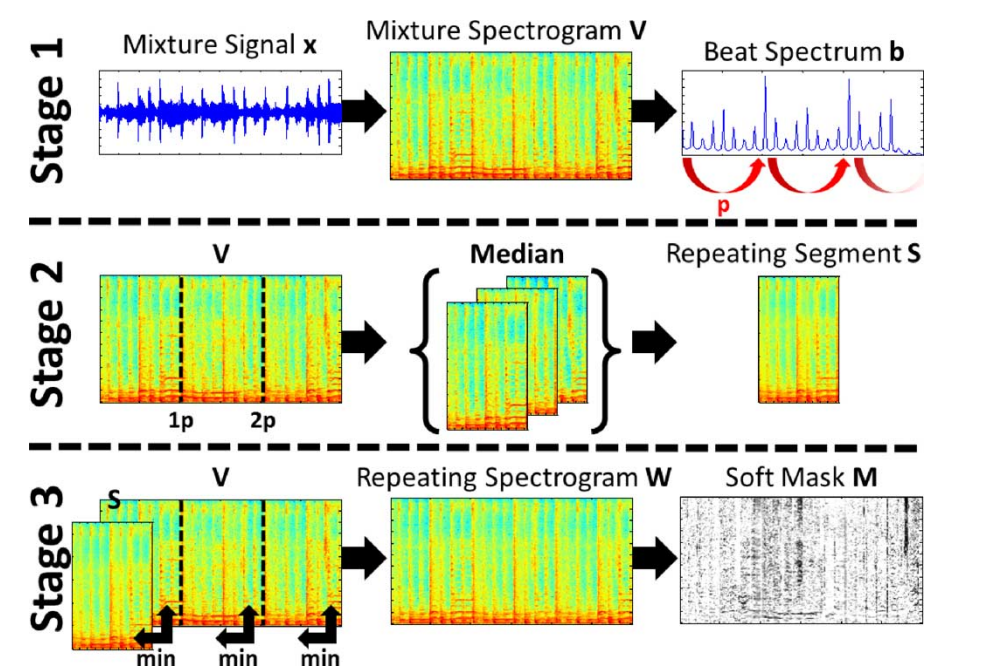
\includegraphics[shift right = 5cm, width=0.5\textwidth]{Figure1.png}\\



This is an example of inserting an equation. 
\begin{equation} \label{eq:first}
    \sum_{i=1}^N  \sum_{d=1}^D (\widetilde{s}_{i, T+d} - {s}_{i, T+d})^2
\end{equation}
The equation Eq.~\ref{eq:first} can be referenced. 


This is an example of inserting a figure. 
\begin{figure}[h]
\begin{center}
%\includegraphics[width=0.5\textwidth]{banner.png}\\
\caption{ This is the banner of ECE 420 webpage.  } 
\label{fig:banner}
\end{center}
\end{figure}
The Figure~\ref{fig:banner} can be referenced. 


This is an example of inserting a table.
\begin{table}[h]
\small
    \centering
    \begin{tabular}{|p{1.5in}|p{1.5in}|}
        \hline
        \textbf{Contents} & \textbf{Number} \\
         \hline
        task1 &  1\\
        \hline
        task2 &  2 \\
         \hline
         
    \end{tabular}
    \vspace{0.1in}
    \caption{Tasks and allocations}
    \label{tab:table}
\end{table}
The Table~\ref{tab:table} can be referenced. 


\section{Plan for testing and validation}
\begin{itemize}
    \item How will you demonstrate it works?
    \item What inputs will you be using?  Are those pre-existing or do they need to be generated?
    \item What are the outputs?  Is it objective or subjective?  Can you collect metrics?
    \item Start with ‘easy’ test cases, work your way up to more complex. 
\end{itemize}

\section{Contribution}
\begin{itemize}
    \item Author 1: task A, B, C
    \item Author 2: task 1, 2, 3
\end{itemize}



 
\bibliographystyle{IEEEtran}
\bibliography{ref}

\end{document}
